\section{Tests de performance}
Para correr los tests de performance se utiliz\'o el paquete \texttt{ubadb.external.bufferManagement} provisto en el
motor para generar trazas v\'alidas que utilizamos como inputs, mediante las clases \texttt{MainEvaluator} y \texttt{MainTraceGenerator}.

Para generar las trazas, utilizamos m\'etodos similares a los implementados en \texttt{MainTraceGenerator}. Esto es
utilizar distintos objetos para generar trazas que simulen accesos normales a una base de datos, siguiente un cierto
patr\'on. Es decir, podemos generar por ejemplo, Filescans de \textit{n} accesos, joins de tipo \textit{BNLJ}, con
tama\~nos parametrizados o accesos a indices del estilo \textit{B+ Tree Clustered} o \textit{Hash}.

Una vez generadas estas trazas corrimos el evaluador (tambi\'en incluido en el c\'odigo) y observamos el
desempe\~no de nuestras implementaciones de single y m\'ultiple buffer pools. Para realizar mediciones m\'as
precisas, comparamos los \textit{hitrates} de acceso a disco considerando casos interesantes de las trazas generadas.
Con esta informaci\'on de los \textit{hitrate}, pudimos generar tablas comparativas que se pueden apreciar en la secci\'on \ref{secTablas}.


\subsection{Resultados de la experimentaci\'on}\label{secTablas}

Fue de interes buscar casos patol\'ogicos para comprobar donde una pol\'itica de
buffers presentara ventajas sobre la otra (buffer compartido vs buffer m\'ultiples).
Nuestra herramienta para comprobar accesos m\'as eficientes es el hitrate,
es decir, cuantas veces se puede acceder a una p\'agina en memoria por cada vez que
la tenemos que acceder a disco. Decimos que el hitrate es ideal cuando
tiende a 100\%, el m\'aximo te\'orico. Entre m\'as alto, mejor.

Una simulaci\'on que hicimos fue una union \texttt{BNLJ} con buffers muy peque\~nos.
Tenemos una tabla de dos p\'aginas, que la marcamos como \texttt{KEEP} y tenemos
una tabla de mil p\'aginas, que la marcamos como \texttt{RECYCLE}.

En total, designamos dos buffer pools con capacidad de dos p\'aginas cada uno
y comparamos contra varios tama\~nos de single buffer pools distintos.

\begin{table}[H]\centering
    \begin{tabular}{l || c}
    \large{\textbf{Estrategia}}                             & \large{\textbf{Hitrate}} [\%] \\
    \hline
    Multiple Buffer Pools KEEP=2 RECYCLE=1 & 49.95       \\
    Single Buffer Pool SIZE=2              & 17.55       \\
    Single Buffer Pool SIZE=4              & 37.70       \\
    Single Buffer Pool SIZE=10             & 48.15       \\
    Single Buffer Pool SIZE=100            & 49.50       \\
    Single Buffer Pool SIZE=200            & 49.70       \\
    \end{tabular}
\end{table}

\begin{figure}[H]\centering
    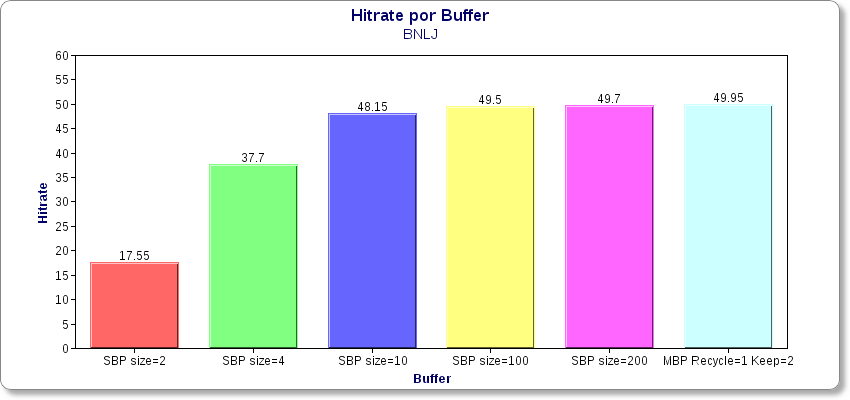
\includegraphics[scale=0.4]{BNLJ.png}
    \caption{Gráfico de Hitrate con respecto a buffer utilizado}
    \label{grafiquito}
\end{figure}

%MANU, SI QUERES HACER GRAFICOS TAN TOP COMO LOS NUESTROS, CLAVATE UN http://www.chartgo.com/. =D =D =D.
%BESITOSSSSSSS Juampi y Juli.

Es decir, solamente con 3 p\'aginas y una administraci\'on inteligente, la eficiencia
de este mecanismo de m\'ultiples buffers supera ampliamente a un buffer pool \'unico de
m\'as de 50 veces el tama\~no.

Otro experimento realizado consistió en los accesos a indices.

Se puede decir que estos experimentos son conociendo el algoritmo del Or\'aculo,
pero es claramente posible comprobarlo en motores reales. Si se contasen
con estadísiticas de uso de las tablas, sería posible asignarles de manera
din\'amica a que pool van a pertenecer cuando se carguen, e incluso es
posible preveer la performance de las operaciones de acuerdo a que pool
se le asigne, considerando como se la va a emplear. Es decir, no estaría
igual de bien asignar una tabla a \texttt{KEEP} si se la va a usar para \textit{filescan}
una sola vez, que asignar a \texttt{KEEP} una tabla que va a ser usada cientos de veces
en un \texttt{BNLJ}.
